% Wenhan's demand section. Compile this self-contained file twice with pdflatex.
% All numerical estimates come from Wenhan's saved v1-v3 outputs.
\documentclass[aspectratio=169,11pt]{beamer}
\usepackage[T1]{fontenc}
\usepackage[utf8]{inputenc}
\usepackage{lmodern,amsmath,amssymb,booktabs,array,tabularx,pgfplots,pgfplotstable}
\usepgfplotslibrary{dateplot}
\pgfplotsset{compat=1.18}
\definecolor{Navy}{HTML}{13294B}
\definecolor{Carolina}{HTML}{4B9CD3}

\definecolor{Slate}{HTML}{596675}
\definecolor{Rust}{HTML}{A94B22}
\definecolor{ScottTeal}{HTML}{007B72}
\definecolor{BrandGray}{HTML}{A2ABB6}
\setbeamercolor{normal text}{fg=Navy,bg=white}
\setbeamercolor{structure}{fg=Carolina}
\setbeamercolor{frametitle}{fg=Navy}
\setbeamerfont{frametitle}{size=\Large,series=\bfseries}
\setbeamersize{text margin left=8mm,text margin right=8mm}
\setbeamertemplate{navigation symbols}{}
\setbeamertemplate{frametitle}{\vspace{3mm}\insertframetitle\par\vspace{1mm}}
\setbeamertemplate{footline}{\hspace{8mm}\color{Slate}\scriptsize ECON 847 PS3\hfill\insertframenumber\hspace{8mm}\vspace{3mm}}
\setbeameroption{hide notes}
\newcommand{\src}[1]{\par\vspace{2mm}{\fontsize{7.3}{8.7}\selectfont\raggedright\color{Slate}#1\par}}
\newcommand{\take}[1]{\par\vspace{2mm}{\bfseries #1}\par}
\newcolumntype{L}[1]{>{\raggedright\arraybackslash}p{#1}}
\title{Bathroom Tissue Demand}
\author{Wenhan Li and Yifan Zhao}
\begin{filecontents*}[overwrite]{brand_shares.csv}
brand,share_pct
ScotTissue,34.88040937014031
Charmin,16.72539174029114
Northern,13.92376522775309
Cottonelle,7.865018735819761
Dominicks,7.037247325109395
Kleenex,5.236133195531941
White Cloud,4.956878511076212
Other brands,9.37515589427815
\end{filecontents*}
\begin{filecontents*}[overwrite]{price_paths.csv}
date,store54,store76,store137
1991-01-03,0.5700,0.5700,0.6200
1991-01-10,0.5700,0.5700,0.6200
1991-01-17,0.5700,0.5700,0.6200
1991-01-24,0.5700,0.5700,0.6200
1991-01-31,0.5700,0.5700,0.6200
1991-02-07,0.5700,0.5700,0.6200
1991-02-14,0.5700,0.5700,0.6200
1991-02-21,0.5700,0.5700,0.6200
1991-02-28,0.5450,0.5450,0.5450
1991-03-07,0.5450,0.5450,0.5450
1991-03-14,0.5700,0.5700,0.6200
1991-03-21,0.5700,0.5700,0.6200
1991-03-28,0.5700,0.5700,0.6200
1991-04-04,0.5400,0.5400,0.5900
1991-04-11,0.5400,0.5400,0.5900
1991-04-18,0.5700,0.5700,0.6200
1991-04-25,0.5700,0.5700,0.6200
1991-05-02,0.5700,0.5700,0.6200
1991-05-09,0.5700,0.5700,0.6200
1991-05-16,0.5700,0.5700,0.6200
1991-05-23,0.5450,0.5450,0.5450
1991-05-30,0.5450,0.5450,0.5450
1991-06-06,0.5700,0.5700,0.6200
1991-06-13,0.5700,0.5700,0.6200
1991-06-20,0.5700,0.5700,0.6200
1991-06-27,0.5700,0.5700,0.6200
1991-07-04,0.5700,0.5700,0.6200
1991-07-11,0.5700,0.5700,0.6200
1991-07-18,0.5700,0.5700,0.6200
1991-07-25,0.5700,0.5700,0.6200
1991-08-01,0.3900,0.3900,0.3900
1991-08-08,0.5700,0.5700,0.6200
1991-08-15,0.5700,0.5700,0.6200
1991-08-22,0.5700,0.5700,0.6200
1991-08-29,0.5700,0.5700,0.6200
1991-09-05,0.5700,0.5700,0.6200
1991-09-12,0.5700,0.5700,0.6200
1991-09-19,0.5700,0.5700,0.6200
1991-09-26,0.5700,0.5700,0.6200
1991-10-03,0.5700,0.5700,0.6200
1991-10-10,0.5700,0.5700,0.6200
1991-10-17,0.3900,0.3900,0.3900
1991-10-24,0.5700,0.5700,0.6100
1991-10-31,0.5700,0.5700,0.6200
1991-11-07,0.5700,0.5700,0.6200
1991-11-14,0.5700,0.5700,0.6200
1991-11-21,0.5700,0.5700,0.6200
1991-11-28,0.5700,0.5700,0.6100
1991-12-05,0.5000,0.5000,0.5000
1991-12-12,0.5600,0.5700,0.6100
1991-12-19,0.5500,0.5500,0.5900
1991-12-26,0.5500,0.5500,0.5900
1992-01-02,0.5500,0.5500,0.5900
1992-01-09,0.5700,0.5700,0.6200
1992-01-16,0.5700,0.5700,0.6200
1992-01-23,0.5700,0.5700,0.6200
1992-01-30,0.5700,0.5700,0.6200
1992-02-06,0.5700,0.5700,0.6200
1992-02-13,0.5700,0.5700,0.6200
1992-02-20,0.5500,0.5500,0.5500
1992-02-27,0.5700,0.5700,0.6200
1992-03-05,0.5700,0.5700,0.6200
1992-03-12,0.5700,0.5700,0.6200
1992-03-19,0.5700,0.5700,0.6200
1992-03-26,0.5000,0.5000,0.5000
1992-04-02,0.5700,0.5700,0.6200
1992-04-09,0.5700,0.5700,0.6200
1992-04-16,0.5700,0.5700,0.6200
1992-04-23,0.5700,0.5700,0.6200
1992-04-30,0.5000,0.5000,0.5000
1992-05-07,0.5700,0.5700,0.6200
1992-05-14,0.5700,0.5700,0.6200
1992-05-21,0.5700,0.5700,0.6200
1992-05-28,0.5700,0.5700,0.6200
1992-06-04,0.5700,0.5700,0.6200
1992-06-11,0.5700,0.5700,0.6200
1992-06-18,0.5000,0.5000,0.5000
1992-06-25,0.5700,0.5700,0.6200
1992-07-02,0.5700,0.5700,0.6200
1992-07-09,0.5700,0.5700,0.6200
1992-07-16,0.5000,0.5000,0.5000
1992-07-23,0.5700,0.5700,0.6200
1992-07-30,0.5600,0.5700,0.5900
1992-08-06,0.5600,0.5600,0.5700
1992-08-13,0.5400,0.5450,0.5400
1992-08-20,0.5400,0.5450,0.5500
1992-08-27,0.5000,0.5000,0.5000
1992-09-03,0.5400,0.5600,0.5700
1992-09-10,0.5100,0.5100,0.6200
1992-09-17,0.5100,0.5100,0.6200
1992-09-24,0.5000,0.5100,0.6100
1992-10-01,0.5000,0.5000,0.5000
1992-10-08,0.5000,0.5000,0.6100
1992-10-15,0.5000,0.5000,0.6100
1992-10-22,0.5000,0.5000,0.6100
1992-10-29,0.5000,0.5000,0.6100
1992-11-05,0.5000,0.5000,0.6000
1992-11-12,0.5000,0.5000,0.6100
1992-11-19,0.5000,0.5000,0.5300
1992-11-26,0.5000,0.5000,0.6000
1992-12-03,0.5000,0.5000,0.6100
1992-12-10,0.5000,0.5000,0.6100
1992-12-17,0.5000,0.5000,0.5400
1992-12-24,nan,nan,0.5400
1992-12-31,0.5000,0.5000,0.5400
\end{filecontents*}
\begin{document}
\begin{frame}{Overview}
\textbf{Project question}\par\vspace{2mm}
How would a hypothetical Scott--Kimberly-Clark merger change bathroom-tissue prices under 1991--1992 conditions?

\vspace{5mm}
The 1995 merger motivates this exercise under 1991--1992 market conditions.\par\medskip

\vspace{5mm}


\begin{columns}[T,onlytextwidth]
\column{.49\textwidth}
\textbf{Wenhan:}
\begin{itemize}\setlength\itemsep{2mm}
\item Industry, markets, and products
\item Data cleaning
\item IV \& Logit
\end{itemize}
\column{.47\textwidth}
\textbf{Yifan:}
\begin{itemize}\setlength\itemsep{2mm}
\item Nested Logit
\item Supply side
\item Merger analysis
\end{itemize}
\end{columns}
\end{frame}
\begin{frame}{Industry}
\small Brands, ply and pack sizes differentiate tissue.
\par\medskip
\begin{columns}[T,onlytextwidth]
\column{.60\textwidth}\centering \textbf{Brand shares}
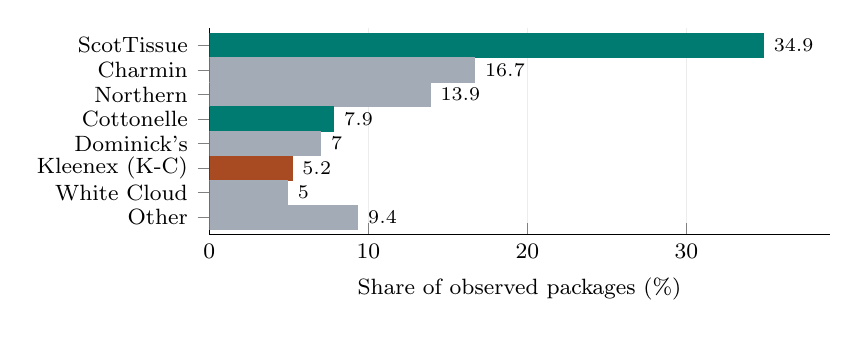
\begin{tikzpicture}
\begin{axis}[width=.78\linewidth,height=42mm,xbar,bar width=3.2mm,xmin=0,xmax=39,
 y dir=reverse,ytick={0,...,7},yticklabels={ScotTissue,Charmin,Northern,Cottonelle,Dominick's,{Kleenex (K-C)},White Cloud,Other},
 yticklabel style={font=\footnotesize},xtick={0,10,20,30},xticklabel style={font=\footnotesize},
 xlabel={Share of observed packages (\%)},xlabel style={font=\footnotesize},
 axis x line*=bottom,axis y line*=left,enlarge y limits=.1,xmajorgrids,grid style={gray!15},
 nodes near coords={\pgfmathprintnumber[fixed,precision=1]{\pgfplotspointmeta}},nodes near coords style={font=\scriptsize,anchor=west},point meta=explicit]
\addplot[fill=ScottTeal,draw=none,bar shift=0pt] coordinates {(34.88040937014031,0) [34.88040937014031]};
\addplot[fill=BrandGray,draw=none,bar shift=0pt] coordinates {(16.72539174029114,1) [16.72539174029114]};
\addplot[fill=BrandGray,draw=none,bar shift=0pt] coordinates {(13.92376522775309,2) [13.92376522775309]};
\addplot[fill=ScottTeal,draw=none,bar shift=0pt] coordinates {(7.865018735819761,3) [7.865018735819761]};
\addplot[fill=BrandGray,draw=none,bar shift=0pt] coordinates {(7.037247325109395,4) [7.037247325109395]};
\addplot[fill=Rust,draw=none,bar shift=0pt] coordinates {(5.236133195531941,5) [5.236133195531941]};
\addplot[fill=BrandGray,draw=none,bar shift=0pt] coordinates {(4.956878511076212,6) [4.956878511076212]};
\addplot[fill=BrandGray,draw=none,bar shift=0pt] coordinates {(9.37515589427815,7) [9.37515589427815]};
\end{axis}\end{tikzpicture}

\column{.37\textwidth}
\raggedright
\textbf{Brands of the merging firms}
\par\medskip
{\color{ScottTeal}\textbf{Scott}\par ScotTissue (34.9\%) and Cottonelle (7.9\%).}
\par\medskip
{\color{Rust}\textbf{Kimberly-Clark}\par Kleenex (5.2\%)}

\end{columns}
\par\vspace{3mm}
\begin{itemize}
    \item 1991--92: 86 stores, 53 UPCs, 8,508 store-weeks. 
    \item Median market: 33 UPCs, 18,675 visits. Median package price: \$1.15.
\end{itemize}
\end{frame}
\begin{frame}{Market and Product Definition}
\small\renewcommand\arraystretch{1.02}
\begin{tabularx}{\textwidth}{@{}L{.18\textwidth}L{.25\textwidth}X@{}}
\toprule
Object & Definition & Economic reason \\
\midrule
Market & Store $\times$ week & Weekly local assortment and pricing decisions. \\
Product & UPC & Distinguishes brands, varieties, and packs. \\
Price / quantity & Dollars per package / packages sold & Aligns the price unit with the sales unit. \\
Market size & Weekly store customer count & Includes shopping opportunities without a tissue purchase. \\
Outside option & No modeled UPC purchased & Allows shoppers to skip the modeled products. \\
\bottomrule
\end{tabularx}\par
\vspace{0mm}
\[
s_{jst}=\frac{\text{\#Packages}_{jst}}{\text{\#Customers}_{st}},
\qquad s_{0st}=1-\sum_j s_{jst}.
\]
\par\vspace{-1mm}\noindent{\normalsize\color{Navy} Shi, Shum, and Song (2018), \emph{Econometrica}.\par Gandhi, Lu, and Shi (2023), \emph{Quantitative Economics}.\par Hausman and Leonard (2002), \emph{Journal of Industrial Economics}.\par}
\end{frame}
\begin{frame}{Data: 1991--1992 Sample and Weekly Prices}
\small
\begin{columns}[T,onlytextwidth]
\column{.43\textwidth}
\textbf{Why 1991--1992?}
\begin{itemize}
\item Relatively stable window before the 1993 Charmin Ultra introduction (Gandhi, Lu, and Shi, 2023).
\item Predates the 1995 Scott--Kimberly-Clark merger.
\end{itemize}
\medskip
\textbf{Why weekly?} Short price dips and reversals are visible within a month. Monthly averages smooth them out.
\column{.54\textwidth}
\centering\textbf{ScotTissue single-roll prices}\par
\begin{tikzpicture}
\begin{axis}[width=.93\linewidth,height=40mm,date coordinates in=x,
 xmin=1991-01-01,xmax=1993-01-01,xtick={1991-01-01,1991-07-01,1992-01-01,1992-07-01,1993-01-01},
 xticklabels={Jan 91,Jul 91,Jan 92,Jul 92,Jan 93},xticklabel style={font=\scriptsize},
 ylabel={Dollars / package},ylabel style={font=\footnotesize},yticklabel style={font=\footnotesize},
 ymin=.30,ymax=.72,ytick={.3,.4,.5,.6,.7},ymajorgrids,grid style={gray!15},axis x line*=bottom,axis y line*=left,
 legend style={font=\scriptsize,draw=none,at={(.5,-.23)},anchor=north,legend columns=3},unbounded coords=jump]
\addplot[Carolina,thick] table[x=date,y=store54,col sep=comma]{price_paths.csv};\addlegendentry{Store 54}
\addplot[Rust,thick,dashed] table[x=date,y=store76,col sep=comma]{price_paths.csv};\addlegendentry{Store 76}
\addplot[Navy,thick,dotted] table[x=date,y=store137,col sep=comma]{price_paths.csv};\addlegendentry{Store 137}
\end{axis}\end{tikzpicture}
\end{columns}
\end{frame}
\begin{frame}{Demand Model: Simple Logit}
\[
\resizebox{.98\linewidth}{!}{$\displaystyle \underbrace{u_{ijst}}_{\text{\scriptsize Utility}} =
\beta_p
\underbrace{p_{jst}}_{\text{\scriptsize Pack price}} +
\underbrace{\mu_{js}}_{\text{\scriptsize Store--UPC FE}} +
\underbrace{\tau_t}_{\text{\scriptsize Week FE}} +
\gamma
\underbrace{D_{jst}}_{\text{\scriptsize Deal flag}} +
\underbrace{\xi_{jst}}_{\text{\scriptsize Demand shock}} +
\underbrace{\varepsilon_{ijst}}_{\text{\scriptsize Taste shock}} .
$}\]
\medskip
\small $i$: shopper, $j$: UPC, $s$: store, $t$: week.
\par\medskip
\begin{itemize}
\item Product characteristics (Brand, pack size, and ply) are constant within a UPC. Their separate coefficients are collinear with store-by-UPC fixed effects.
\item Store-by-UPC fixed effects absorb persistent differences in product quality and local preferences.
\item Follow Shi, Shum, and Song (2018, \emph{Econometrica}).
\end{itemize}
\smallskip
\textbf{Estimation.} FE-OLS provides the benchmark. FE-2SLS uses each instrument separately and treats the recorded deal flag as exogenous.
\end{frame}
\begin{frame}{IV}
\textbf{AAC (average acquisition cost).}
\[
p-\mathrm{AAC}=p\times\underbrace{\frac{\mathrm{PROFIT}}{100}}_{\text{gross margin rate}}.
\]
\small
\begin{itemize}\setlength{\itemsep}{0pt}
\item \textbf{Relevance.} Retail prices respond to acquisition costs.
\item \textbf{Exclusion.} Manufacturer promotions may link acquisition costs to local demand shocks.
\item \textbf{Reference.} Gandhi, Lu, and Shi (2023).
\end{itemize}
\textbf{Other-store price.} Same UPC and week, using at least five other stores.
\begin{itemize}\setlength{\itemsep}{0pt}
\item \textbf{Relevance.} Common costs can move prices across stores.
\item \textbf{Exclusion.} Shared promotions may link other-store prices to local demand shocks.
\item \textbf{Reference.} Hausman and Leonard (2002).
\end{itemize}
\textbf{External input cost shifters:} weak first-stage evidence.
\end{frame}
\begin{frame}{IV First Stage}
\[\underbrace{\widetilde p_{jst}}_{\text{Pack price}} =
\pi_z\underbrace{\widetilde z_{jst}}_{\text{Price IV}} +
\pi_D\underbrace{\widetilde D_{jst}}_{\text{Deal flag}} +
\underbrace{v_{jst}}_{\text{Residual}}.\]
\small\centering\renewcommand\arraystretch{1.10}
\begin{tabular}{@{}lrr@{}}
\toprule
 & AAC & Other-store price \\
\midrule
Excluded-instrument coefficient & $0.394$ & $0.990$ \\
Clustered SE & $(0.036)$ & $(0.027)$ \\
\midrule
Partial $R^2$ & $0.125$ & $0.721$ \\
Excluded-IV Wald $\chi^2(1)$ & $119.35$ & $1{,}324.90$ \\
Observations & 277,363 & 276,820 \\
\bottomrule
\end{tabular}\par
\end{frame}
\begin{frame}{Logit Results}
\small\centering\renewcommand\arraystretch{1.2}
\begin{tabular}{@{}lrrrr@{}}
\toprule
 & OLS (no FE) & FE OLS & AAC-IV & Other-store-IV \\
\midrule
Price coefficient & $-0.409$ & $-2.111$ & $-2.107$ & $-2.582$ \\
Clustered SE & $(0.016)$ & $(0.123)$ & $(0.324)$ & $(0.161)$ \\
Store--UPC / week FE & No & Yes & Yes & Yes \\
Median own elasticity & $-0.47$ & $-2.42$ & $-2.42$ & $-2.96$ \\
Inelastic observations & 86.70\% & 2.26\% & 2.28\% & 0.29\% \\
Observations & 277,363 & 277,363 & 277,363 & 276,820 \\
\bottomrule
\end{tabular}\par

\par\medskip\raggedright
FE-OLS and AAC-IV give similar price coefficients. Other-store IV implies the largest absolute median own-price elasticity.
\end{frame}
\end{document}